\documentclass[letterpaper]{article} % DO NOT CHANGE THIS
\usepackage{aaai2027}  % DO NOT CHANGE THIS
\usepackage[hyphens]{url}  % DO NOT CHANGE THIS
\usepackage{graphicx} % DO NOT CHANGE THIS
\urlstyle{rm} % DO NOT CHANGE THIS
\def\UrlFont{\rm}  % DO NOT CHANGE THIS
\Urlmuskip=0mu plus 2mu  % let long URLs in the references stretch instead of overfilling the column
\usepackage{natbib}  % DO NOT CHANGE THIS AND DO NOT ADD ANY OPTIONS TO IT
\usepackage{caption} % DO NOT CHANGE THIS AND DO NOT ADD ANY OPTIONS TO IT
\frenchspacing  % DO NOT CHANGE THIS
\usepackage{booktabs}
\usepackage{amsfonts}
\usepackage{amsmath}
\graphicspath{{./}}
\usepackage{xr}
\makeatletter
\newcommand*{\addFileDependency}[1]{\typeout{(#1)}\@addtofilelist{#1}\IfFileExists{#1}{}{\typeout{No file #1.}}}
\makeatother
\newcommand*{\myexternaldocument}[1]{\externaldocument[][nocite]{#1}\addFileDependency{#1.tex}\addFileDependency{#1.aux}}
\myexternaldocument{supplement}
\pdfinfo{
/TemplateVersion (2027.1)
}
\setcounter{secnumdepth}{0}
\nocopyright

\title{Black--Scholes for the Land:\\ Modelling Weather-Adjusted Savanna Response as an Invertible Transition-Density World Model}
\author{
    Thomas Pitts\textsuperscript{\rm 1},
    Yu Luo\textsuperscript{\rm 2},
    Chuancheng Shi\textsuperscript{\rm 2},
    Bin Liang\textsuperscript{\rm 1},
    Zhiyong Wang\textsuperscript{\rm 2}
}
\affiliations{
    \textsuperscript{\rm 1}University of Technology Sydney\\
    \textsuperscript{\rm 2}University of Sydney\\
    thomas.pitts@uts.edu.au
}

\begin{document}
\maketitle

\begin{abstract}
Vegetation growth in rangeland is fundamental to the issuance of soil carbon credits, but disentangling the impacts of weather, such as rainfall, from those of grassland management practices is an open problem. Incumbent baselines rely on mean annual rainfall to calculate carbon capture, ignoring the season's weather, while residual-trend methods regress linearly on annual rain. We propose an invertible transition-density world model conditioned on rain and evaporative demand, and used as Black--Scholes is used in options pricing. Inverted on observed greenness it yields an implied residual, i.e. the land's weather-adjusted response; rolled forward under other drivers it can generate counterfactuals; and differentiated with respect to its drivers and state it gives sensitivities, close analogues of the Black--Scholes Greeks. On unseen years 2019--25, the $\Delta$ of our model (the derivative of greenness with respect to rain) has an error of $22\%$ on average across 2.2\,km blocks, close to the $19\%$ year-to-year noise floor, while swapping the model's backbone for Chronos-2, a 120M-parameter time-series foundation model, yields an error of $80\%$. Our model's residual shows no detectable weather bias, neither rewarding wet seasons nor penalising dry ones. In the 2022 drought in Laikipia, Kenya, the land fell $0.168$ NDVI below normal---our model attributes $63\%$ of that drop to the weather, not the land manager.

\end{abstract}

\begin{figure*}[t]
\centering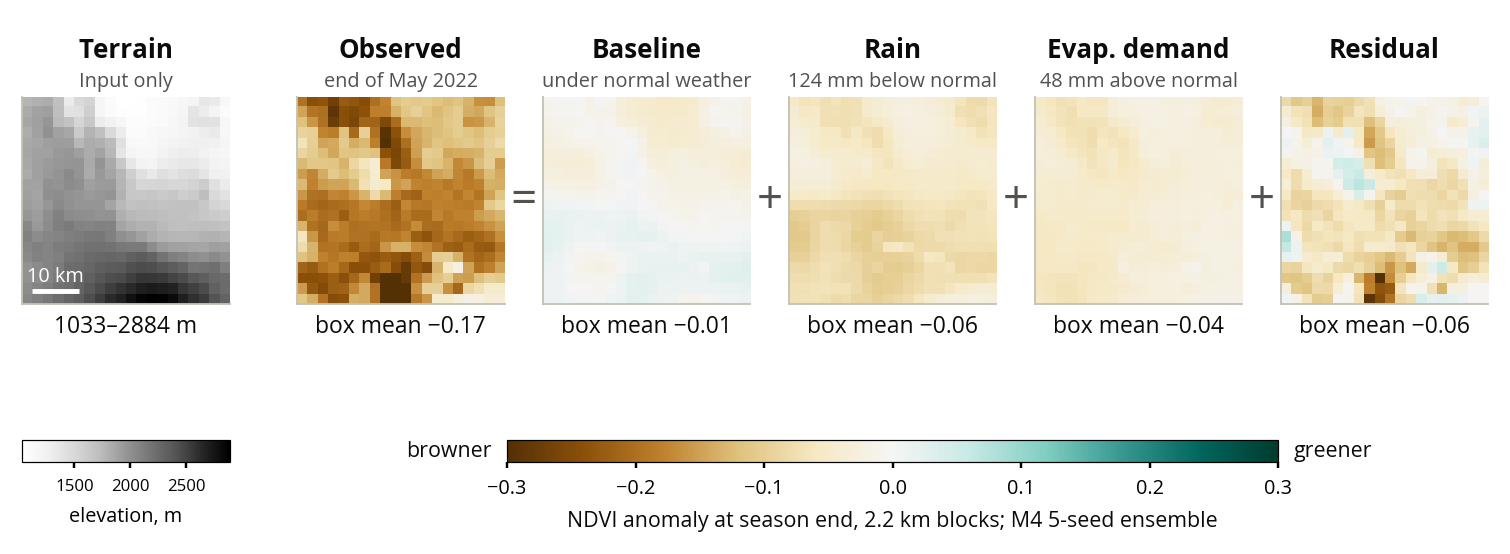
\includegraphics[width=\textwidth]{fig_maps_split_2022_m4e.png}
\caption{Box A, March--May 2022, a held-out year. Season-end NDVI anomaly per 2.2\,km block from M4. Every run starts from the late-February state with residual zero. The baseline is the run under normal weather. Rain and evaporative demand split the run under the weather that fell minus the baseline by Shapley value. The residual is observed minus that run. Elevation, left, is an input and not a share.}
\label{fig:split}
\end{figure*}

\section{Introduction}
To monitor and validate efficacy of sustainable grassland management practices such as rotation of grazing animals, replanting strategies, and backburning, it is critical to establish accurate carbon capture measurements. The Northern Kenya Rangelands Carbon Project, the world's largest soil carbon removal project, earns one credit per tonne of CO$_2$ stored in soil above a baseline set by VM0032, a pioneering grazing methodology \citep{vm0032,verra2023}. However, that baseline was contested enough for Verra to suspend issuance for eight months in 2023 \citep{verra2023}. Its baseline model, SNAP \citep{ritchie2014,nkgcp_pd2016}, uses only mean annual rainfall, rather than an input such as CHIRPS 16-day periodic rainfall \citep{chirps} or even seasonal rain records. Without a reliable mechanism to disentangle major drivers of land surface greenness i.e. the normalised difference vegetation index (NDVI),  a farmer who changes nothing can then be penalised for the effects of dry seasons they did not cause, or rewarded for wet seasons. Fine-grained NDVI attribution should encourage the sustainable practices that materially contribute to increased carbon capture. To the best of our knowledge, no current operational baseline makes that split cleanly.

% Elsewhere, livestock index insurance in the same counties pays on seasonal NDVI against the insured area's own history \citep{deoto2019}. For maximum efficiency, the insurer ideally would want to quantify forage loss attributed only to factors specifically included in the policy, such as drought, rather than management decisions such as overgrazing. Both categories of payment would benefit from a clean split of the land's response between the climatic conditions and other remaining factors. To the best of our knowledge, no current operational baseline makes that split cleanly. 

In this work we propose a model that makes that split with climate factors as its conditioning input, specifically, CHIRPS rain and ERA5 evaporative demand (ED) \citep{hersbach2020}, two key drivers of the climatic water balance \citep{spei} in these rangelands. We also show that adding static attributes \citep{kratzert2019} materially improves the model's skill in forecasts over single-step (16 days) and 3-month timeframes, by adding in topography in the form of Copernicus DEM GLO-30 elevation, slope, and topographic position \citep{copdem}. The residual this leaves, the land's response net of the weather, is a cleaner signal of management than greenness alone.

Our approach is borrowed from the Black--Scholes formula (BSF) \citep{bs}, which is used to price an option from observables (the stock price, strike, time to expiry and interest rate) and one unobservable parameter, the volatility. By instead inverting on the actual market price, the BSF produces ``implied'' volatility. In our model, the observables are the land's current state and the rain and ED that fell. Inverted on the observed greenness, the model produces the part of the land's response the weather does not explain. We term this weather-adjusted response the \textbf{implied residual}. By feeding in other weather, \textbf{counterfactual scenarios} can be modelled, and per-pixel patch \textbf{sensitivities} can be derived by automatic differentiation through the model rollout.

Our contributions are as follows:
\begin{itemize}
    \item An invertible transition-density world model of greenness, with the weather as the action, whose inversion gives the implied residual.
    \item Greek-like sensitivities derived by differentiating through the model rollout, which can stand in for the full model: a $\Delta$-weighted sum of observed weather anomalies recovers the weather term to first order in droughts, and to second order with $\Gamma$ in wet seasons, where greenness saturates.
    \item A finding that good forecasting does not imply an accurate world model of the land, shown with the Chronos-2 time-series foundation model.
\end{itemize}


\section{Related Work}

Existing approaches to separating weather effects from that of land management fall into three groups. The first adjusts for rainfall by linear regression. Residual trend analysis (RESTREND) regresses NDVI on rainfall for each pixel and interprets a declining trend in the residual, the component the regression does not explain, as human-induced degradation \citep{evans2004}. Vegetation sensitivity indices add the previous month's greenness as a predictor \citep{seddon2016}. In East Africa, however, greenness responds to the rainfall of the current and two preceding months and saturates in wetter areas \citep{davenport1993}, a response that a linear model cannot represent. We retain the residual but replace the regression with a learned model of how greenness evolves over each 16-day step given the weather.

The second group makes no adjustment for weather. Livestock insurance in Kenya scores each season's greenness against the same area's historical record as a z-score \citep{vrieling2014,deoto2019}. A low score indicates a poor season but cannot distinguish drought from management as its cause.

The third group comprises time-series foundation models, large networks pretrained on diverse series. These produce full predictive distributions \citep{chronos2}, and one has forecast leaf area index without task-specific training \citep{zhang2025}. Such models are designed for forward prediction. To our knowledge, none are built to be inverted on observations or re-run under another driver path.

\begin{figure*}[t]
\centering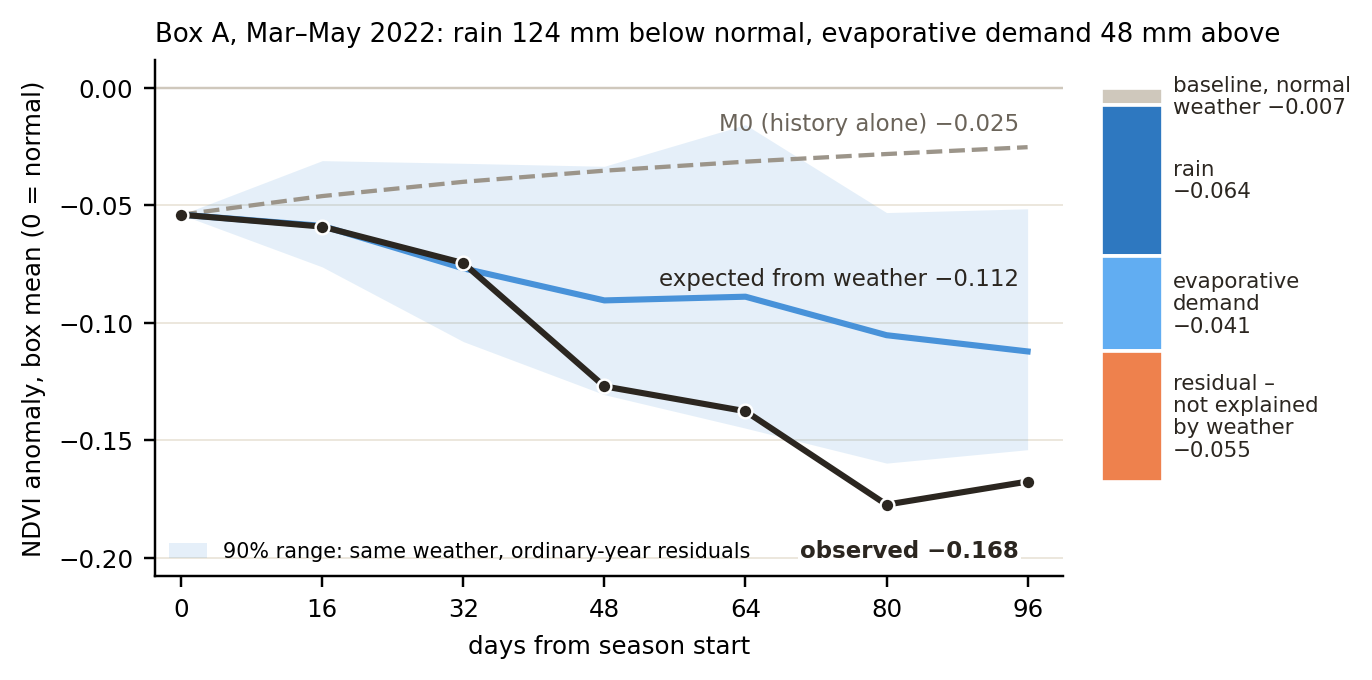
\includegraphics[width=\textwidth]{fig_2022_attribution_m4.png}
\caption{The 2022 drought, Box A, a held-out year: box means from M4, with the expected path run at zero residual. Shading as in the Appendix. Right: the season-end split by \eqref{eq:split}.}
\label{fig:attribution}
\end{figure*}

\section{Methodology}

\paragraph{Model} Our model is a world model in the sense of the memory model M of \citet{ha2018}: a predictive model of the future that outputs a probability density function. Our model estimates the specific terrain response from data as a transition density for the greenness anomaly $a$ in place of their learned latent state $z$, given a water-balance memory $w$ of past climatic water balance rather than a recurrent memory $h$, and its current weather value $u$ in place of the agent's action $\mathrm{act}_t$.
\begin{alignat*}{4}
\text{\citet{ha2018}, M:}\quad & p_\theta(z_{t+1} &&{}\mid z_t,\; && h_t,\; && \mathrm{act}_t)\\
\text{Ours:}\quad & p_\theta(a_{t+1} &&{}\mid a_t,\; && w_t,\; && u_{t+1})
\end{alignat*}


Each step sees only the current state, not the series i.e. Markovian. The state is the anomaly $a_t$ and an antecedent index $w_t$ of the climatic water balance, a one-parameter bucket whose memory $\lambda(x)$ depends on the pixel's traits:
\begin{align}
w_{t+1} &= \lambda(x)\,w_t + u_{t+1}, \nonumber\\
a_{t+1} &= a_t + \mu_\theta(a_t, \bar a_t, w_t, u_{t+1}, \phi_{t+1}, x) \nonumber\\
&\quad + \sigma_\theta(\cdot)\,\varepsilon_t,\qquad \varepsilon_t\sim\mathcal N(0,1),
\label{eq:model}
\end{align}
where $t$ indexes 16-day steps, $\bar a_t$ is the $5\times5$ neighbourhood mean of $a_t$, $\phi_{t+1}$ is the seasonal phase (sine and cosine of day of year), $x$ is six static traits of the pixel: mean NDVI, seasonal amplitude, climatological annual rain, and elevation, slope and topographic position from the Copernicus GLO-30 DEM \citep{copdem}, and $u_t=r_t-k(x)\,e_t$ is rain net of ED, the climatic water balance \citep{spei}, with $k$ linear in the traits. $w_t$ is a decaying sum of past $u_t$ that keeps a fraction $\lambda(x)=\mathrm{sigmoid}(c_0+c^\top x)$ each step. $\mu_\theta$ is the expected change in the anomaly and $\sigma_\theta$ its spread, both functions of the same six inputs, so $p_\theta(a_{t+1}\mid\cdot)=\mathcal N(a_t+\mu_\theta,\sigma_\theta^2)$; $\theta$ is one set of weights shared by every pixel. \textbf{M0} uses history alone. \textbf{M1} has $\mu$ and $\log\sigma$ linear in the features. \textbf{M2} adds a 64-unit one-hidden-layer network to $\mu$ and $\log\sigma$. \textbf{M3} adds the topographic traits to M2. \textbf{M4} adds ED ($k=0$ below M4) to M3 and is an equal-weight mixture of five fits. All are fitted by full-batch Adam on the one-step Gaussian log-likelihood of observed transitions.

\paragraph{Residual} Inverting \eqref{eq:model} on an observed transition gives the implied (standardised) residual,
\begin{equation}
\hat\varepsilon_t = \frac{a_{t+1} - a_t - \mu_\theta(a_t,\bar a_t,w_t,u_{t+1},\phi_{t+1},x)}{\sigma_\theta(\cdot)},
\label{eq:implied}
\end{equation}
which in practical terms is simply one number per pixel per 16 days, in units of the model's predicted standard deviation, $\sigma_\theta$. Each step is a one-layer conditional affine flow \citep{papamakarios2021}, so the model is invertible: each observed transition has a unique residual. Here $F_h$ is \eqref{eq:model} rolled forward from the season's starting state with zero residual along the observed rain and ED. Carried autoregressively through the rollout, the implied residuals reproduce the observed path exactly, so their combined effect is the residual term for the season, $a_{t+h}-F_h$, in NDVI rather than units of $\sigma_\theta$. We produce an interval for $F_h$ by re-running the season with residuals resampled from the training seasons (Figure~\ref{fig:attribution}). 


\paragraph{Counterfactual} 

Rolled along any other weather path $(r',e')$, $u'=r'-k(x)\,e'$, the same rollout gives $F_h(r',e')$, so $F_h=F_h(r,e)$. With $(\bar r,0)$, $\bar r$ being the climatological rain, each pixel's 2003--2018 mean for that 16-day step of the year, and $0$ a zero ED anomaly, the season-end anomaly splits exactly into baseline, weather and residual,
\begin{equation}
\medmuskip=1.5mu\thickmuskip=2.5mu
a_{t+h}=\underbrace{F_h(\bar r,0)}_{\text{baseline}}+\underbrace{[F_h(r,e)-F_h(\bar r,0)]}_{\text{weather term}}+\underbrace{[a_{t+h}-F_h(r,e)]}_{\text{residual}}.
\label{eq:split}
\end{equation}
The weather term is divided between rain and ED by Shapley value over the four combinations of observed and normal rain and ED \citep{shapley1953} (Figure~\ref{fig:split}). 

\paragraph{Sensitivities}
Following the BSF Greeks, we take Jacobian-vector products through the rollout at normal weather: $\Delta_h=\partial F_h(\bar r,0)/\partial r_{t+1}$, greenness $h$ steps ahead per $100$\,mm of rain now. $\Gamma_h=\partial^2F_h(\bar r,0)/\partial r_{t+1}^2$ is a measure of the saturation effect, or rather, how the sensitivity of $\Delta$ itself changes with rain. $\Theta_h=\partial F_h(\bar r,0)/\partial a_t$ is a measure of how long it takes for anomalies or shocks to subside.

\section{Experiments \& Results}

\paragraph{Data} The target $a_t$ is greenness, the normalised difference vegetation index (NDVI) from the MODIS satellite product MOD13Q1 \citep{mod13}, at $250$\,m every 16 days (one composite), 2002--2025, as an anomaly against each pixel's 2003--2018 climatology. The z-score, the incumbent standard in index insurance, divides this anomaly by the pixel's standard deviation for that time of year; we quote it undivided, in NDVI, for direct comparison. The input $r_t$ is rain from CHIRPS \citep{chirps} summed over the same 16-day windows, in units of $100$\,mm; $e_t$ is ED, FAO-56 reference evapotranspiration \citep{allen1998} from ERA5 \citep{hersbach2020}, likewise summed, as an anomaly against 2003--2018. The setting is two $45$\,km savanna regions in Laikipia, Kenya, with seasonal rains typically in March--May and October--December: Box A (development) and Box B (held-out landscape) to its west (Figure~\ref{fig:map}, Appendix). We fit on Box A 2003--2017, early-stop on 2018, and evaluate on 2019--2025 for both boxes. This evaluation period is 13 seasons, including a drought in 2021--22 and the subsequent 2023 recovery.


\begin{figure}[t]
\centering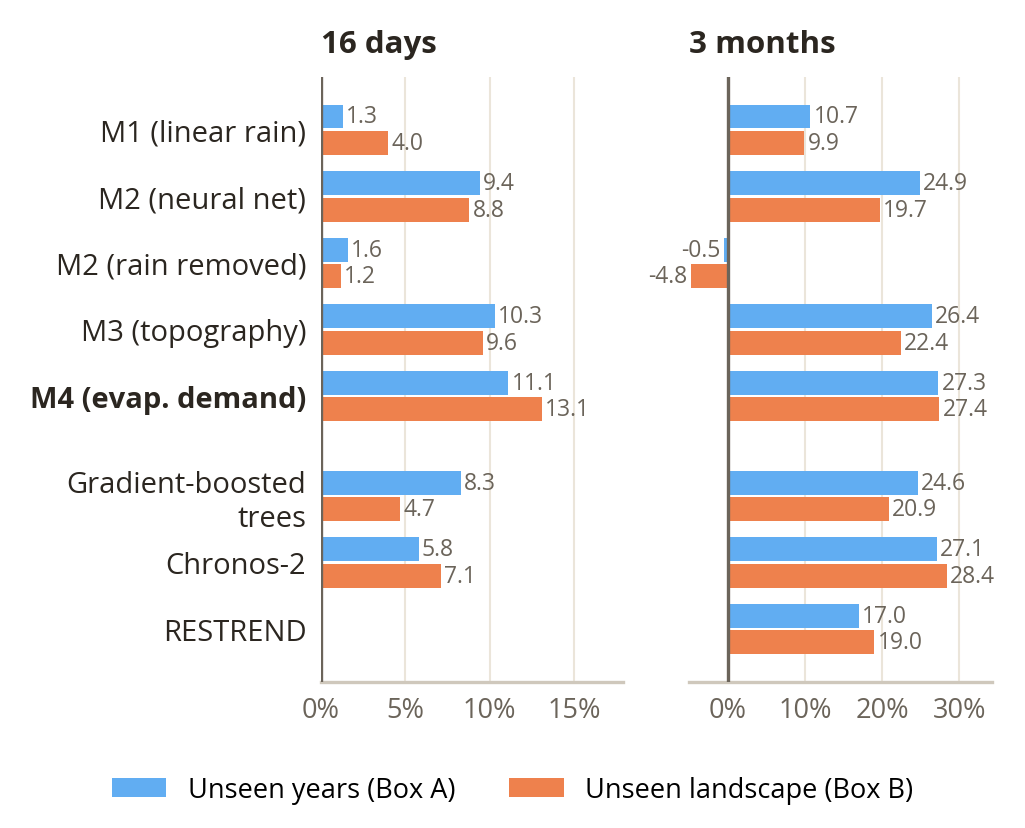
\includegraphics[width=\columnwidth]{fig_skill_c2.png}
\caption{Error reduction against history alone (M0), as CRPS skill on held-out years 2019--25, one step (16 days) and six steps (3 months) ahead along the weather that occurred. M2, M3 and M4 are five-fit ensembles; M2 (rain removed) is a single-seed fit. RESTREND gives season-end values only. Chronos-2 runs zero-shot on 4,000 sampled pixels.}
\label{fig:skill}
\end{figure}

\paragraph{Evaluation} Error is the continuous ranked probability score (CRPS) \citep{gneiting2007}, the probabilistic generalisation of absolute error, on observed held-out pixel-steps (one pixel at one 16-day composite); skill is $1-\mathrm{CRPS}/\mathrm{CRPS}_{\mathrm{M0}}$. Each model is scored one step (16 days) ahead, and rolled forward 3 months along the observed weather. As the canonical machine-learning baseline we also fit gradient-boosted trees (GBT) \citep{friedman2001} on recent greenness, rain, ED and the pixel's traits, including topography. We also compare our model to Amazon's Chronos-2 \citep{chronos2}, a time-series foundation model representative of the current state of the art. Chronos-2 is given each pixel's full history from 2002 up to the forecast date and, like our models, the rain and ED that actually fell over the forecast window.

\begin{table}[t]\centering\footnotesize\setlength{\tabcolsep}{4pt}
\caption{The March--May 2022 drought, Box A, held out. The season-end anomaly of $-0.168$ NDVI split by \eqref{eq:split}, box means. Time is for the full-box split: Chronos-2 on one H100 GPU, the others on a laptop CPU.}\label{tab:drought}
\begin{tabular}{lrrrr}\toprule
 & z-score & RESTREND & Chronos-2 & M4\\\midrule
Baseline & -- & -- & $+.003$ & $-.007$\\
Rain & -- & $-.075$ & $-.014$ & $-.064$\\
ED & -- & -- & $-.088$ & $-.041$\\
\textbf{Weather} & $\mathbf{.000}$ & $\mathbf{-.075}$ & $\mathbf{-.102}$ & $\mathbf{-.105}$\\
\textbf{Residual} & $\mathbf{-.168}$ & $\mathbf{-.092}$ & $\mathbf{-.069}$ & $\mathbf{-.055}$\\\midrule
Parameters & -- & 76,800 & 120M & 5,010\\
Time & 0.1\,ms & $<$0.1\,ms & 11\,min & 71\,ms\\\bottomrule
\end{tabular}
\end{table}

\begin{figure*}[t]
\centering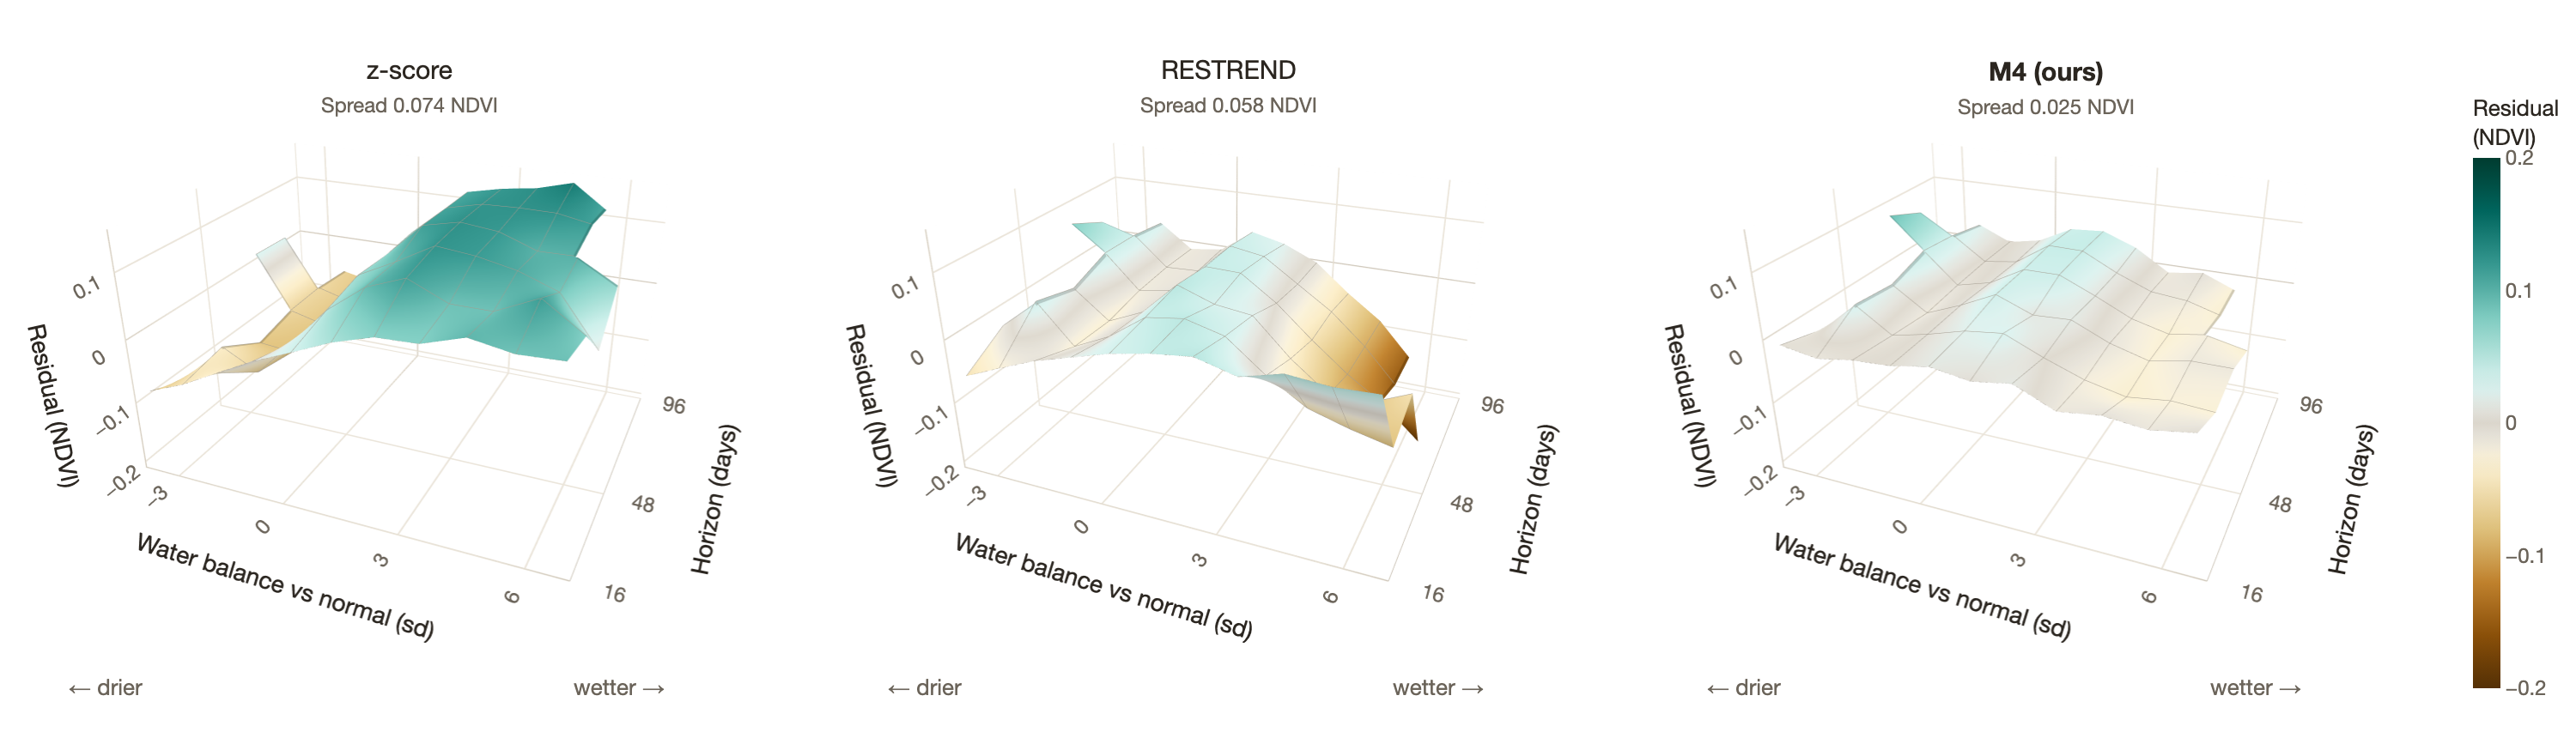
\includegraphics[width=\textwidth]{plotly_faceted_row.png}
\caption{Implied residual surface, Box A, held-out years 2019--25 (141 start dates). Each cell is the mean residual over 2.2\,km blocks, by horizon and by the water-balance departure since the start (rain minus ED, in standard deviations). In unseen years, the z-score tilts with the weather while RESTREND bends, primarily in the wet tail. M4 remains broadly flat. Spread is the standard deviation of the cell means; cells with fewer than three years are omitted.}
\label{fig:surface}
\end{figure*}

\paragraph{Fit}Adding drivers consistently yields increased skill, at both horizons and on both landscapes (Figure~\ref{fig:skill}, Table~\ref{tab:onestep}). For comparison, we run M2 with and without rain, showing that almost all of its skill is predicated on the rain data. Topography (M3) adds $1$--$3$ points, and ED (M4) under one point on unseen years but $3.5$--$5$ on the unseen landscape, the more arid of the two boxes, where we theorise evaporative demand to have a higher influence. Along the weather that fell, M4's 3-month skill is $27$ points above history and $10$ above RESTREND on unseen years, and it beats GBT in every column. Against Chronos-2, a 120M-parameter foundation model given the same weather, M4 nearly doubles the 16-day skill and comes within a point at 3 months, with 5,010 parameters.

\paragraph{Residual} 
In March--May 2022 the land leaves the range ordinary years' residuals give (shading, Figure~\ref{fig:attribution}) only in the last month of the season, while M0, forecasting from history alone, expects recovery and ends above that range.

\begin{figure}[t]
\centering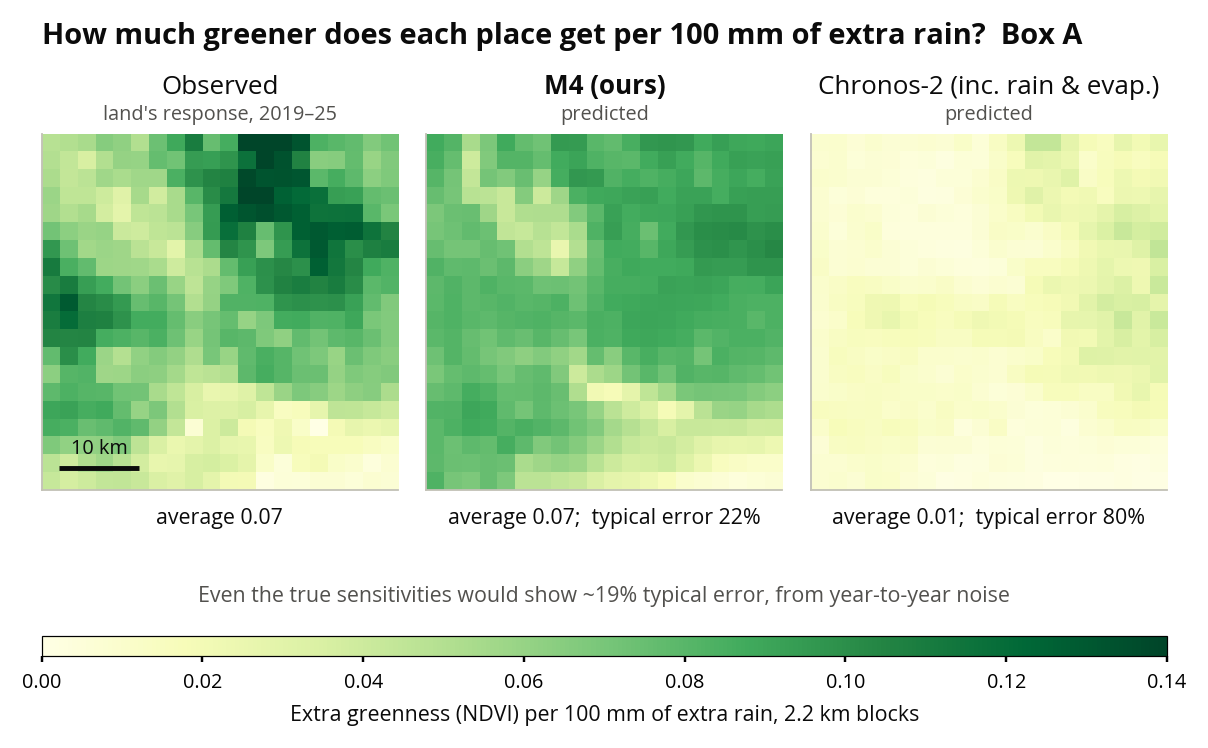
\includegraphics[width=\columnwidth]{fig_sens_c2.png}
\caption{$\Delta$ per 2.2\,km block, Box A, unseen years 2019--25. Left, the observed response, the NDVI change two steps on per $100$\,mm of rain anomaly, given starting greenness. Middle, the M4 ensemble's mean $\Delta$ over the same starts. Right, Chronos-2, given the same weather, on 4,000 sampled pixels.}\label{fig:sens}
\end{figure}

The implied residual surfaces, analogous to implied volatility surfaces, are shown for the z-score, RESTREND, and M4 in Figure~\ref{fig:surface} for the unseen years on Box A. Under Black--Scholes, the implied volatility surface would theoretically be perfectly flat. In reality, surfaces often exhibit skew, as well as anomaly spikes and troughs. Likewise, an implied residual surface free of weather should be flat along the water-balance axis, and any slant is weather left in it. Across all 141 held-out start dates and horizons up to 3 months, the z-score's residual tilts noticeably with the water balance, while RESTREND's bends in the wet tail due to the mismatch between linear projection and the saturation effect of rain on growth. 

Meanwhile, M4's lack of slant illustrates the neutrality of its residual relative to weather: it does not reward wet seasons or penalise dry ones. Across 13 held-out seasons it moves $+0.004$ NDVI per $100$\,mm of climatic water balance (rain minus ED, with $95\%$ interval $-0.005$ to $+0.022$), against $+0.040$ for a z-score (Table~\ref{tab:bias}). RESTREND also shows no detectable bias ($-0.008$), but its linearity causes issues at the extremes. In the wettest season, October--December 2019, it overshoots, predicting $48\%$ above the highest box mean in its training data, and leaves a $-0.133$ NDVI residual, against $-0.018$ for M4. In other words, M4 is extracting the weather's nonlinear effect on the land.

\paragraph{Counterfactual}

The counterfactual re-runs the same season from the same starting state under normal weather, and is the mechanism by which we can compute attribution per driver. In March--May 2022 the box ended $0.168$ NDVI below normal (Figure~\ref{fig:attribution}, Table~\ref{tab:drought}). A z-score, the basis of current livestock index insurance, attributes all of it to the land. M4 attributes $0.105$ to the weather. Run through the same split with Chronos-2 as the backbone, the weather share is $0.102$, within the $0.091$--$0.114$ range of M4's five fits.

\paragraph{Sensitivities}

\textit{$\Delta$ and $\Gamma$, rain sensitivity.} On the box mean, an extra $100$\,mm of rain raises greenness by $0.072$ NDVI a month later. Per 2.2\,km block on unseen years, M4's $\Delta$ is off the observed response by $22\%$ on average, against $19\%$ for a perfect model given year-to-year noise, $37\%$ for a flat map at the box mean and $80\%$ for Chronos-2 (Figure~\ref{fig:sens}). Recomputed from the current state at each rainy-season step, $\Delta$ also tracks when a patch responds. Within each pixel, steps in the top $\Delta$ third green $2.8$ times as much per $100$\,mm as those in the bottom third (Table~\ref{tab:greeks}). On the unseen landscape the ranking does not hold, within pixels or across them (Table~\ref{tab:greekstests}).

To first order, the weather term of \eqref{eq:split} can alternatively be expressed as the departures from normal weather, weighted by $\Delta$,
\begin{equation}
\underbrace{F_h(r,e)-F_h(\bar r,0)}_{\text{weather term}}\approx\underbrace{\textstyle\sum_s \Delta^{r}_{h,s}\,\delta r_s}_{\text{rain}}+\underbrace{\textstyle\sum_s \Delta^{e}_{h,s}\,\delta e_s}_{\text{ED}},
\label{eq:taylor}
\end{equation}
where $\delta r_s,\delta e_s$ are the departures of rain and ED from normal in window $s$ and $\Delta^r_{h,s}=\partial F_h/\partial r_s$, $\Delta^e_{h,s}=\partial F_h/\partial e_s$ are taken at normal weather from the pre-season state ($\Delta_h=\Delta^r_{h,t+1}$). In every gap-free held-out drought it is within $8\%$ of the full rollout. In wet seasons greenness saturates: the rain curvature $\Gamma=\partial^2F_h/\partial r^2$ is negative in every held-out season, and adding the second-order terms brings the approximation within $4\%$ in every season more than $100$\,mm wetter than normal (Table~\ref{tab:taylor}). Having quantified $\Delta$ per pixel for a given season, a contract can define the weather's share of the season through a simple weighted sum of rain and ED departures, with no model run needed.

\textit{$\Theta$ and $\partial\sigma/\partial r$, decay and spread.} The same rollout quantifies how fast a shock to greenness decays, and how much rain widens the spread of outcomes. We leave further exploration of both to future work.

\section{Discussion}

\paragraph{Limitations} The evidence comes from two $45$\,km boxes in one region and 13 held-out seasons. The residual separates weather from everything else: it also holds fire, unmodelled weather and sensor noise, so crediting it to management assumes those average out. This is not yet validated against recorded management. We leave further drivers, and feedbacks such as weather-driven grazing decisions, to future work.

\paragraph{World model} How can a model with 5,010 parameters match a 120M-parameter pretrained foundation model on skill yet beat it three-fold on $\Delta$? The difference is a structural one between the two paradigms: world models, and time-series forecasters. Residuals and counterfactuals depend on how the model responds to its drivers. This is not the same as being a good forecaster. Good forecasting along the weather that actually occurred does not necessarily require a correct response to each driver. Chronos-2 matches M4 at 3-month skill, yet its $\Delta$ is $80\%$ off the observed response against M4's $22\%$ (Figure~\ref{fig:sens}) and its ranking of patches by sensitivity is backwards ($-0.047$ NDVI per $100$\,mm, most minus least sensitive third, against M4's $+0.061$ on the same pixels).

We cannot inspect Chronos-2's internals, but we posit one possibility based on the data. Across seasons, rain and ED move almost in lockstep (correlation $-0.98$), so a forecaster can lean on either driver, and Chronos-2 does indeed lean on ED, splitting the 2022 drought mostly to ED (Table~\ref{tab:drought}). At a 16-day step however, the correlation is only $-0.5$, and in a typical fortnight rain differs by about $60$\,mm across the box, while ED varies only by about $3$\,mm. In other words, within a given fortnight, ED acts like a constant while rain varies across pixels. M4 on the other hand is forced to learn a single transition for all $25\,600$ pixels, conditioned on each pixel's terrain and state, so must be able to explain why pixels a few km apart have different outcomes in the same timeframe. A forecaster reading one pixel's series at a time, even its entire recorded history, never sees those differences.

\section{Conclusion}
Inverting our learned transition-density world model on observed satellite data produces the implied residual, the land's weather-adjusted response, and with it the weather's impact, the two sides that carbon credit issuance needs. Its counterfactuals separate that share from the land's starting state and break it down by driver, demonstrated here with rain and ED. By differentiation, the model derives each pixel's sensitivity to rain, which ranks response on unseen years. While run only as a proof of concept on limited data, we believe invertible transition-density world models have potential for complex real-world temporal systems and welcome further exploration in this space.

\bibliography{references}
\end{document}
